\documentclass[11pt,a4paper]{article}
\usepackage{ucs}
\usepackage[T1]{fontenc}
\usepackage[utf8x]{inputenc}
\usepackage[german]{babel}
\usepackage{amsmath}
\usepackage{amsfonts}
\usepackage{amssymb}
\usepackage{graphicx}
\usepackage{shadethm}
\usepackage{caption}
\usepackage{tikz} 
\usepackage{ziffer}
\usepackage{units}
\usepackage{multirow}
\usepackage{subfigure}
\usepackage{hyperref}
\usepackage{cleveref}

\newcommand{\minipanf}{\begin{minipage}{\linewidth}}
\newcommand{\minipend}{\end{minipage}}
\newcommand{\abs}[1]{\ensuremath{\left\vert#1\right\vert}}

\begin{document}

\begin{titlepage}
\newcommand{\HRule}{\rule{\linewidth}{0.5mm}} % Defines a new command for the horizontal lines, change thickness here

\center % Center everything on the page
 
%----------------------------------------------------------------------------------------
%	HEADING SECTIONS
%----------------------------------------------------------------------------------------

\textsc{\LARGE TU Dresden}\\[1.5cm] % Name of your university/college
\textsc{\Large Fortgeschrittenenpraktikum}\\[0.5cm] % Major heading such as course name
\textsc{\Large Praktikumsbericht}\\[0.5cm] % Major heading such as course name

%----------------------------------------------------------------------------------------
%	TITLE SECTION
%----------------------------------------------------------------------------------------

\HRule \\[0.7cm]
{ \huge \bfseries Lebensdauer von Myonen}\\[0.4cm] % Title of your document
\HRule \\[1.5cm]
 
%----------------------------------------------------------------------------------------
%	AUTHOR SECTION
%----------------------------------------------------------------------------------------

\begin{minipage}{0.4\textwidth}
\begin{flushleft} \large
\emph{Autoren:}\\
Toni \textsc{Ehmcke}\\
Christian \textsc{Siegel}
\end{flushleft}
\end{minipage}
~
\begin{minipage}{0.4\textwidth}
\begin{flushright} \large
\emph{Betreuer:} \\
Maximilian \textsc{Hils} % Supervisor's Name
\end{flushright}
\end{minipage}\\[4cm]

%----------------------------------------------------------------------------------------
%	DATE SECTION
%----------------------------------------------------------------------------------------

{\large Dresden, \today}\\
\vspace{5mm}
{\large Durchführungstag, 08. Januar 2016}\\

\vfill 

\end{titlepage} 	% Titelseite

\tableofcontents
\newpage 

\section{Einführung}

	\subsection{Entstehung von Myonen}
	\textit{Myonen} $\mu{\pm}$ lassen sich im heute gängigen Standardmodell der Teilchenphysik zur zweiten Generation der elektrisch geladenen Leptonen zuordnen. Sie sind mit $m_\mu = 105,658\ \unit{MeV = 206,768\ m_e}$\cite{pdg} die schweren Pendants zum Elektron.\\
	Im folgenden Versuch werden Myonen aus der kosmischen Höhenstrahlung, welche zu 85\% aus hochenergetischen Protonen besteht, untersucht. Bei Zusammenstößen dieser Protonen mit Atomkernen in der Erdatmosphäre entstehen die geladenen $\pi^\pm$-Mesonen Reaktionen niedrigster Ordnung sind:
		\begin{align*}
			&p + p \longrightarrow p + n + \pi^+\\
			&p + n \longrightarrow p + p + \pi-
		\end{align*}
	Diese Mesonen zerfallen nach etwa $2,6\cdot10^{-8}\ \unit{s}$ über die schwache Wechselwirkung. Der mit einem Anteil von 99,988\% dominierende Zerfallskanal endet in einem Myon und einem zugehörigen Neutrino und kann mit folgender Zerfallsgleichung und dem Feynmandiagramm in Abbildung \ref{fig:pionzerfall} beschrieben werden:
		\begin{align*}
			&\pi^+ \longrightarrow \mu^+ + \nu_\mu\\
			&\pi^- \longrightarrow \mu^- + \bar{\nu}_\mu\\
		\end{align*}
		\begin{figure}[hp]
					\centering
					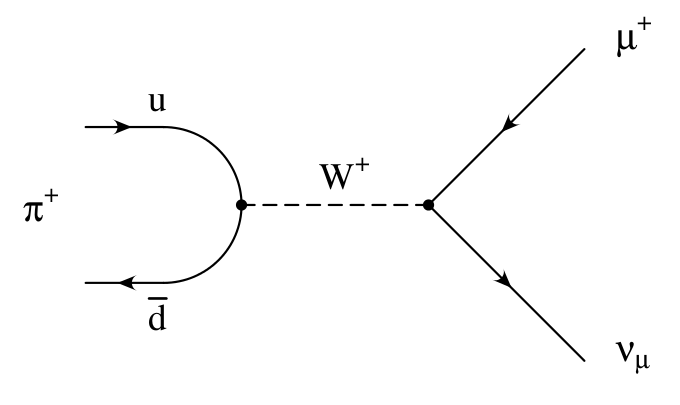
\includegraphics[width = 0.7\linewidth]{pic/pionzerfall.png}
					\caption{Feynman-Diagramm des Antimyonenzerfalls.}
					\label{fig:pionzerfall}
		\end{figure}
		
	\subsection{Zerfall von Myonen}
	Da das Myon ein sehr schweres Teilchen ist, zerfällt es nach einer sehr kurzen Zeit von:\cite{PA}\\
		\begin{equation} \label{eq:lit}
			\tau_\mu = (2,19703 \pm 0,00004)\ \unit{\mu s}
		\end{equation}
	mit nahezu 100\% über den schwachen Zerfall, der mit Hilfe der Reaktionsgleichungen (\ref{eq:mup}) und (\ref{eq:mum}) und zugehörigem Feynmangraph (nur niedrigste Ordnung) in Abbildung \ref{fig:myonzerfall} beschrieben werden kann.\\
	
		\begin{align}
			&\mu^+ \longrightarrow e^+ + \nu_e + \bar{\nu}_\mu 		\label{eq:mup}\\
			&\mu^- \longrightarrow e^- + \bar{\nu}_e + \nu_\mu 		\label{eq:mum}
		\end{align}
		\begin{figure}[hp]
			\centering
			\scalebox{0.5}[0.5]{
			\input{pic/myonzerfall.pdf_tex}
			}
			\caption{Feynman-Diagramm des Antimyonenzerfalls.}
			\label{fig:myonzerfall}
		\end{figure}
	\ \\
	Auch wenn die in Gleichung (\ref{eq:lit}) angegebene Lebensdauer sehr kurz erscheint, ist der Myonenfluss auf Meereshöhe mit $170\ \unit{Myonen/(m^2s)}$ sehr hoch. Dies lässt sich dadurch erklären, dass die oben angegebene Lebensdauer im Laborsystem der Beobachter auf der Erde angegeben ist. Da sich Myonen mit relativistischen Energien bewegen, besitzen sie in ihrem Ruhesystem eine \textit{zeitdilatierte Lebensdauer}, welche ausreicht, um an die Erdoberfläche zu gelangen. Selbst in der theoretischen Vorhersage der Lebensdauern mit Hilfe von \textit{Übergangsmatrixelementen} $\Gamma_{fi} = 1/\tau_{fi}$ (d.h. bei Übergang von Zustand $\ket{i}$ in $\ket{f}$) treten Terme auf, die nicht lorentzinvariant sind.
	
	\subsection{$\mu^-$-Einfang}
	Im Falle der negativ elektrisch geladenen Myonen $\mu^-$ existiert in Materie allerdings ein weiterer 'Zerfallskanal', der sogenannte $\mu^-$-Einfang, bei dem ein einfallendes Myon im Coulombfeld eines Atoms eingefangen wird, bis in den Grundzustand vordringt und anschließend vom Kern absorbiert wird. Dabei findet folgende Kernumwandlung(Abbildung \ref{fig:myoneinfang}) statt:
		\begin{equation*}
			\mu^- + p \longrightarrow  \nu_\mu + n 
		\end{equation*}
		
		\begin{figure}[ht]
			\centering
			\scalebox{1.}[1.]{
			\input{pic/myoneneinfang.pdf_tex}
			}
			\caption{Feynman-Diagramm des Myoneneinfangs.}
			\label{fig:myoneinfang}	
		\end{figure}
	\ \\
	Ist $\Gamma_z = 1/\tau_z$ die Partialbreite  des schwachen Zerfallskanals (\ref{eq:mum}) und $\Gamma_e=1/\tau_e$ die des $\mu^-$-Einfangs, ergibt sich die totale Breite des $\mu^-$-Zerfalls zu:
		\begin{align}
			&\Gamma_{\mu^-} = \Gamma_z + \Gamma_e\\
			&\tau_{\mu^-} = \left(\frac{1}{\tau_z} + \frac{1}{\tau_e}\right)^{-1} < \tau_{\mu^+}  
		\end{align}
	Im Praktikumsversuch werden die Myonen mit einer Kupferplatte eingefangen. Da der $\mu^-$-Einfang dafür sorgt, dass nach etwa $1\ \unit{\mu s}$ alle negativ geladenen Fermionen eingefangen worden, dominieren die $\mu^+$-Zerfälle die Messung. 
	
	\subsection{Messprinzip und Versuchsaufbau}
    \begin{figure}
        \centering 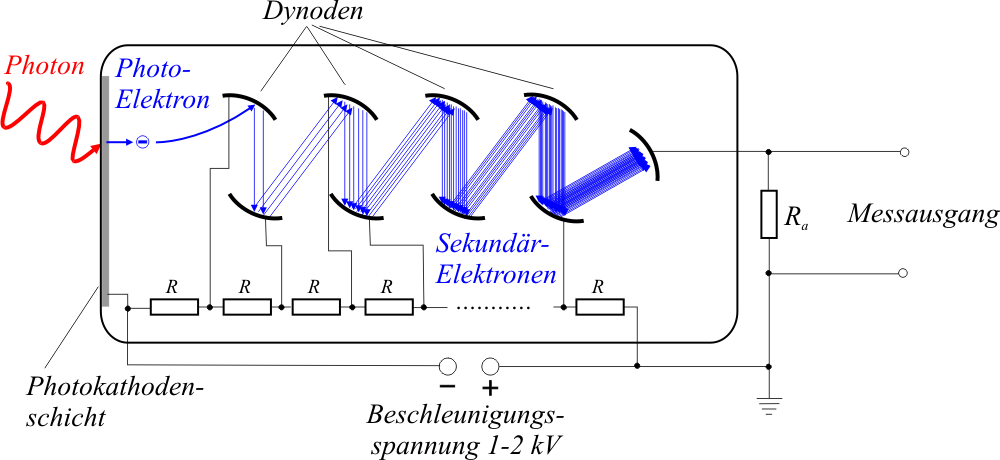
\includegraphics[scale=0.85]{pic/pm.png}
        \caption{\cite{pm} Skizze des Aufbaus eines PM}
    \end{figure}
	%TODO@Christian: Kurz beschreiben wie Szintillator und PM funktioniert + Versuchsaufbau (nur Messaufbau 1)		% Physikalischer Hintergrund
\section{Durchführung}
    \subsection{Vorversuche Gruppe B, LM1}
        Bevor mit dem Hauptversuch begonnen werden kann, müssen diverse Vorversuche durchgeführt werden, um die Versuchsparameter zu optimieren.
        \subsubsection{Aufnahme der Kennlinie von Photomultiplier 3 (PM3)}
            Als erstes soll nach Aufgabenstellung die Kennlinie des PM3 aufgenommen werden. Dafür muss zunächst die Messtechnik angeschlossen werden. In diesem Versuch wurde das Koinzidenzsignal (1·2·3) auf den Counter 1 und das einfache Signal 3 auf den Counter mit der Nummer 2 gelegt.\\
            Danach stellt man die Hochspannungen für die Multiplier 1 und 2 ($U_{1,HV}$ und $U_{2,HV}$) auf jeweils etwa $\unit[2400]{V}$ ein. Danach wird die Hochspannung für Photomultiplier 3 auf etwa $2100\unit{V}$ geregelt. Diese Gruppe erreichte für PM1 $U_{1,HV} = 2403\unit{V}$, für $U_{2,HV} = 2401\unit{V}$ und für $U_{3,HV} = 2099\unit{V}$. 
            Nun erfolgt die Evaluierung der Messdauer. Dafür muss zunächst über den relativen Fehler ermittelt werden, wie viele Counts gemessen werden sollen. 
            $$ \frac{\Delta N}{N} = N^{-\frac{1}{2}} \leq 3\unit{\%}$$
            Da die Counts poisson-verteilt sind, erhält man für $\Delta N = \sqrt{N}$. Die Zahl der zu messenden Ereignisse (Counts) ergibt sich über diese Rechnung zu 1112. Nun wählt man im Messprogramm die Option ab, die Messung nach einer bestimmten Zeit anzuhalten und misst solange, bis Counter 1 ungefähr den errechneten Wert erreicht, wobei zu beachten ist, dass der gemessene Wert größer ist, um den relativen Fehler unterhalb der $3\unit{\%}$ zu halten. Diese Gruppe hat für einen Counter-Wert von 1122 eine Messdauer $t_{Mess} = 117\unit{s}$ gemessen. Diese Zeit wird für die Aufnahme der Kennlinie benötigt.
            Für die Aufnahme der Kennlinie des PM3 wird die Spannung $U_{3,HV}$ in $50\unit{V}$-Schritten von $1800\unit{V}$ bis $2400\unit{V}$ variiert. Die Stufen werden $t_{Mess}$ lange gemessen. 
            \begin{figure}[htbp]
                \subfigure[Kennlinie des PM3 mit Signal $N_{1·2·3}$\label{n123}]{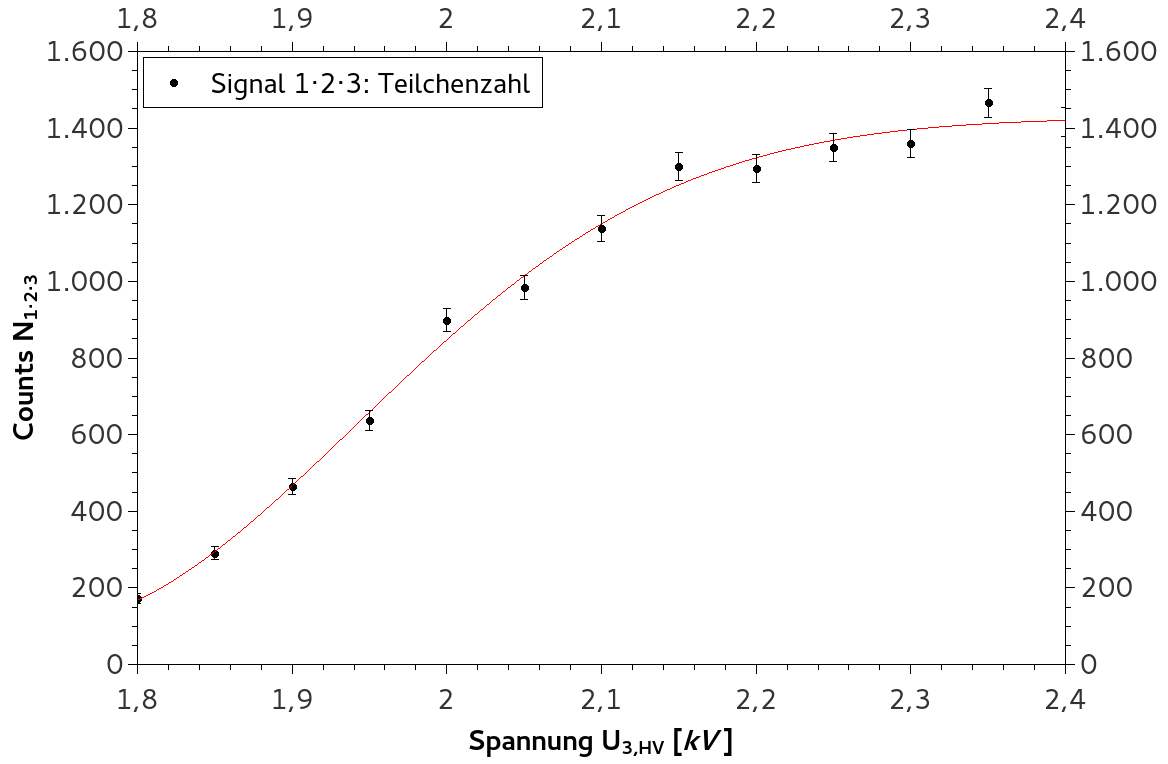
\includegraphics[scale=0.225]{pic/n123u3th}}
                \subfigure[Kennlinie des Signals $N_3$\label{n3}]{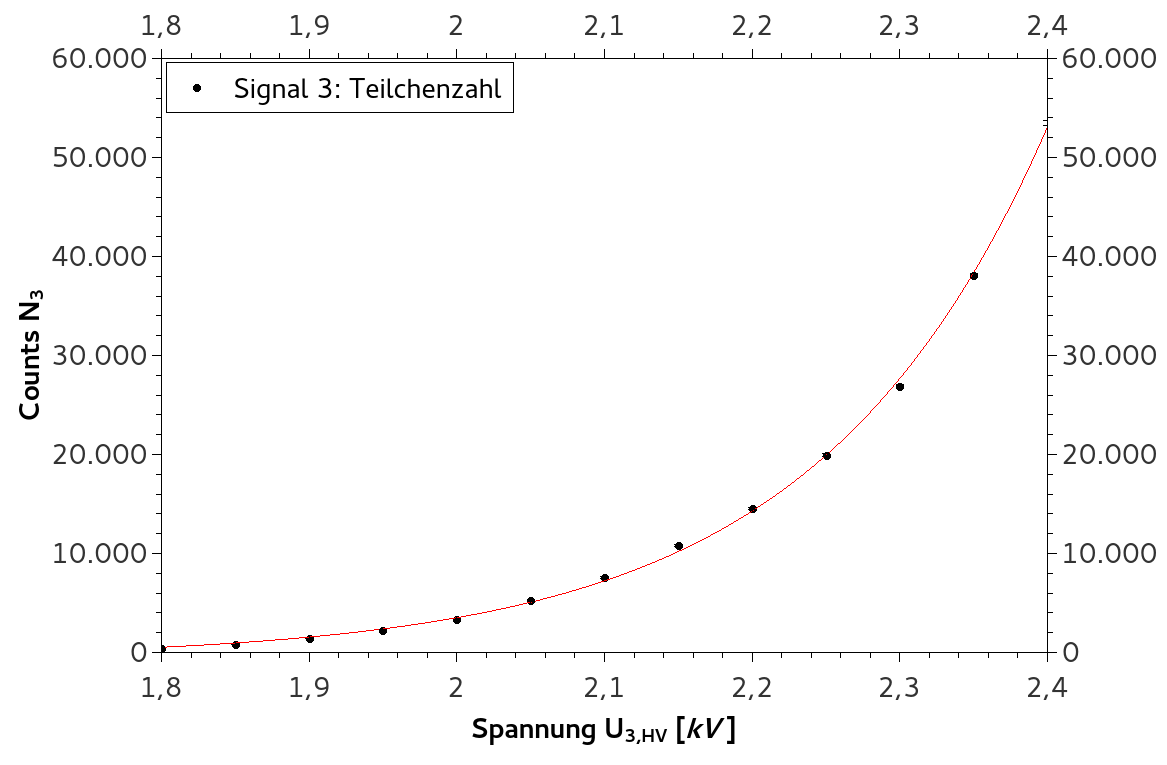
\includegraphics[scale=0.225]{pic/n3u3th}}
                \caption{Kennlinien der Hochspannung $U_{3,HV}$}
            \end{figure}
            Die Abbildungen \ref{n123} und \ref{n3} sehen sehr verschieden aus. Es ist stark auffällig, dass es sich bei \ref{n3} um ein exponentielles Wachstum handelt, während sich in \ref{n123} ein Plateau herausbildet, dessen verhalten eher einer kummulativen Verteilungsfunktion der Gauß-Kurve ähneln. 
            Die Unterschiede rühren vorallem daher, dass in \ref{n123} eine Triplezählrate vorliegt, für die Signale von allen Photomultipliern notwendig sind, um einen Count zu zählen. Es werden nur Signale gezählt, die in das Koinzidenzzeitfenster fallen und den Detektor in einer bestimmten, oben genannten Reihenfolge durchlaufen. In \ref{n3} handelt es sich um eine Singlezählrate, die nur den Photomultiplier 3 misst, dessen Hochspannung man verändert. Es wird kein Koinzidenzzeitfenster beachtet und es werden alle ankommenden Signale, bis auf das Signalrauschen, welches durch einen Diskriminator herausgefiltert wird, gemessen. Mit den steigenden Spannungen werden aus den im PM verbauten Dynoden mehr Elektronen herausgeschlagen. Damit steigt die Vervielfachung erheblich.\\
            Aus \ref{n123} kann man die Schwellspannung $U_{3,Schwell} = 2250\unit{V}$ ablesen. Sie wird als Optimierungsparamter im Hauptversuch benötigt.
        \subsubsection{Messung von Myon-Pulsen}
    \subsection{Hauptversuch}
        Für diesen Versuchsteil benötigt man die Schwellspannungen der einzelnen Photomultiplier. $$ U_{1,Schwell} = 2400\unit{V};\ U_{2,Schwell} = 2400\unit{V};\ U_{3,Schwell} = 2250\unit{V} $$. Die Schwellspannung von PM1 und PM2 wurden von Gruppe A ermittelt und an alle Gruppen weitergegeben. Sie sind durch Ablesen von den Kennlinien-Diagrammen (vgl. Abb. \ref{n123}) mit Fehlern behaftet, die das Experiment nachhaltig beeinflussen können.
        Interessant sind die Diskriminatorspannungen $U_{n,D}$ der PM, da sie das Signalrauschen unterdrücken sollen. Sie liegen bei: $$ U_{1,D} = 200\unit{mV};\ U_{2,D} = 200,5\unit{mV};\ U_{3,D} = 200,6\unit{mV} $$
        Die Messdauer beträgt 5 Tage, das heißt $t_{Mess} = 5\cdot24\cdot60\cdot60\unit{s} = 432000\unit{s}$			% Durchführung
%\section{Zusammenfassung und Diskussion}

\newpage
\section{Anhang}
In diesem Abschnitt findet sich das handschriftlich erstellte Messprotokoll mit der uns gegebenen Aufgabenstellung.\\
\begin{figure}[htbp]
    \subfigure[Aufgabenstellung]{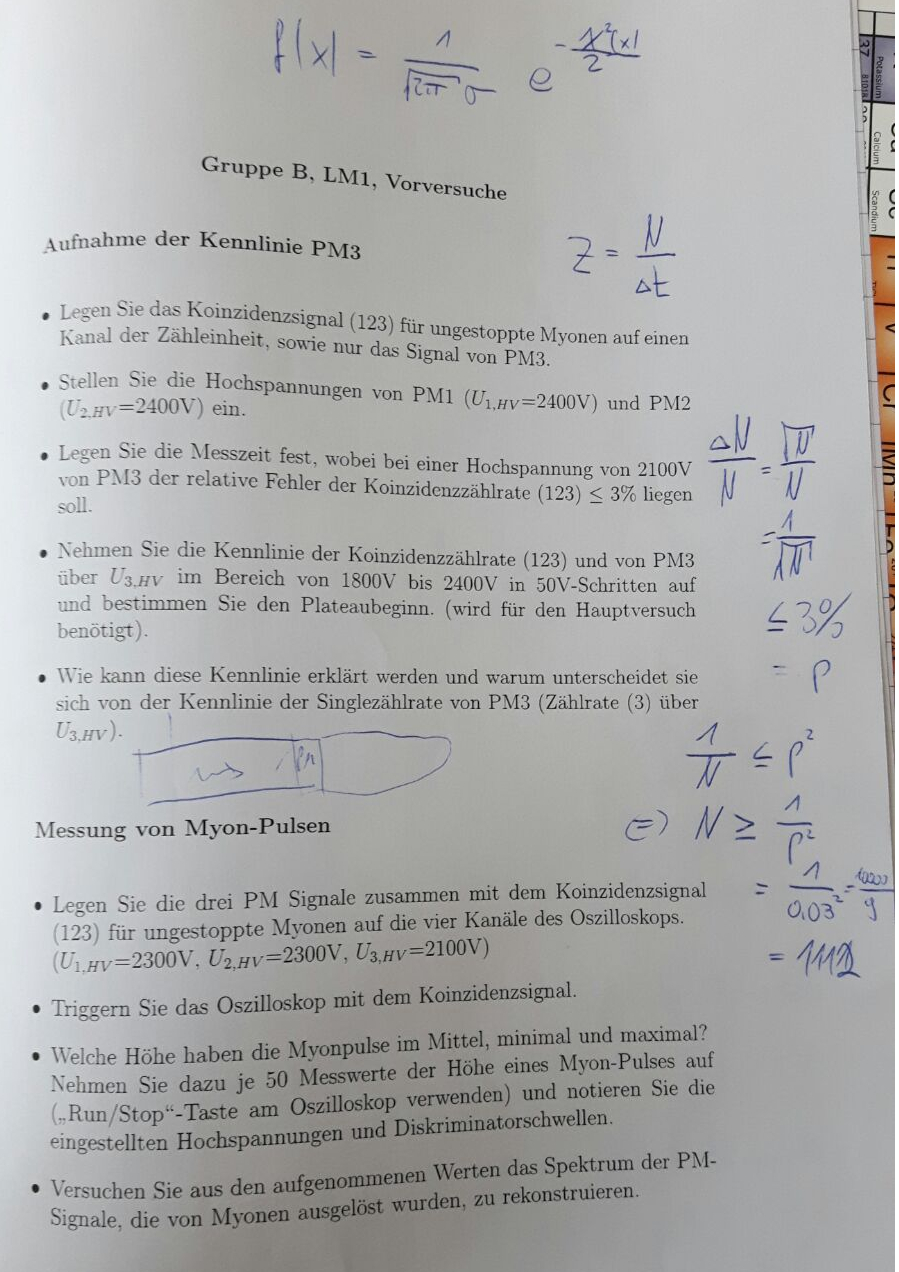
\includegraphics[scale=0.6]{pic/aufgabe.jpg}}
    \subfigure[S1, handschrftl. MP]{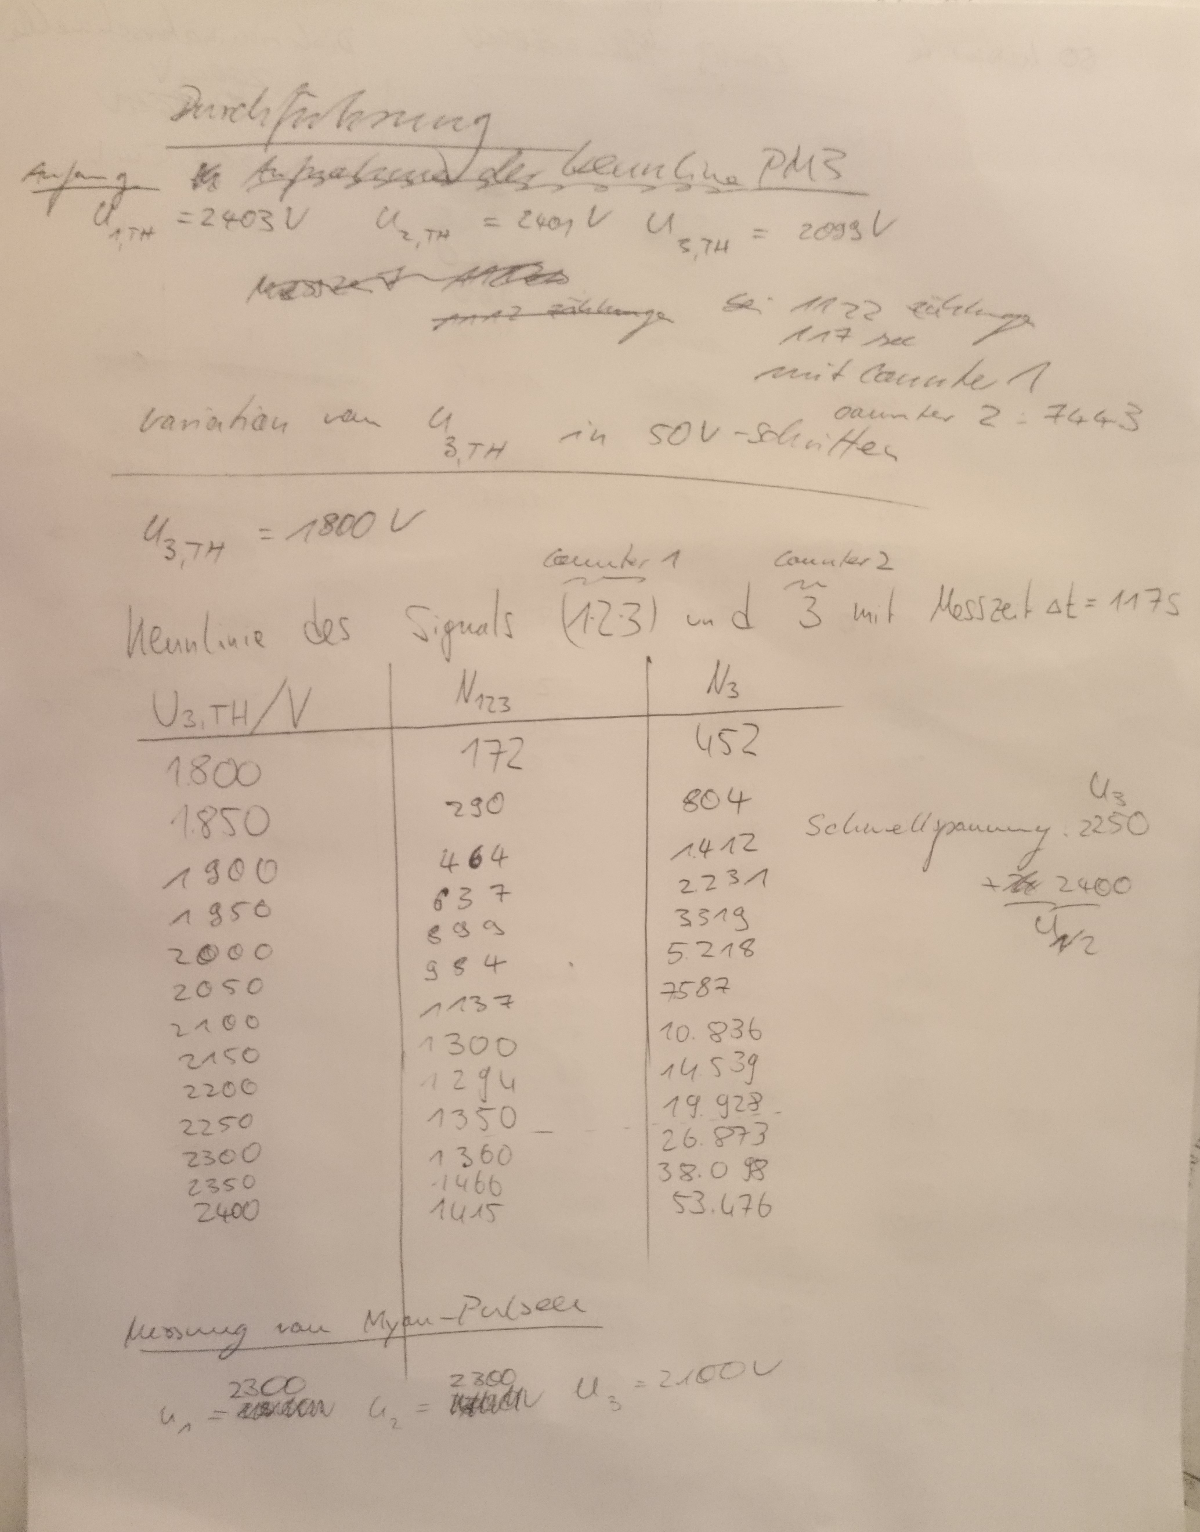
\includegraphics[scale=0.12]{pic/mess1.png}}
    \centering \subfigure[S2, handschiftl. MP]{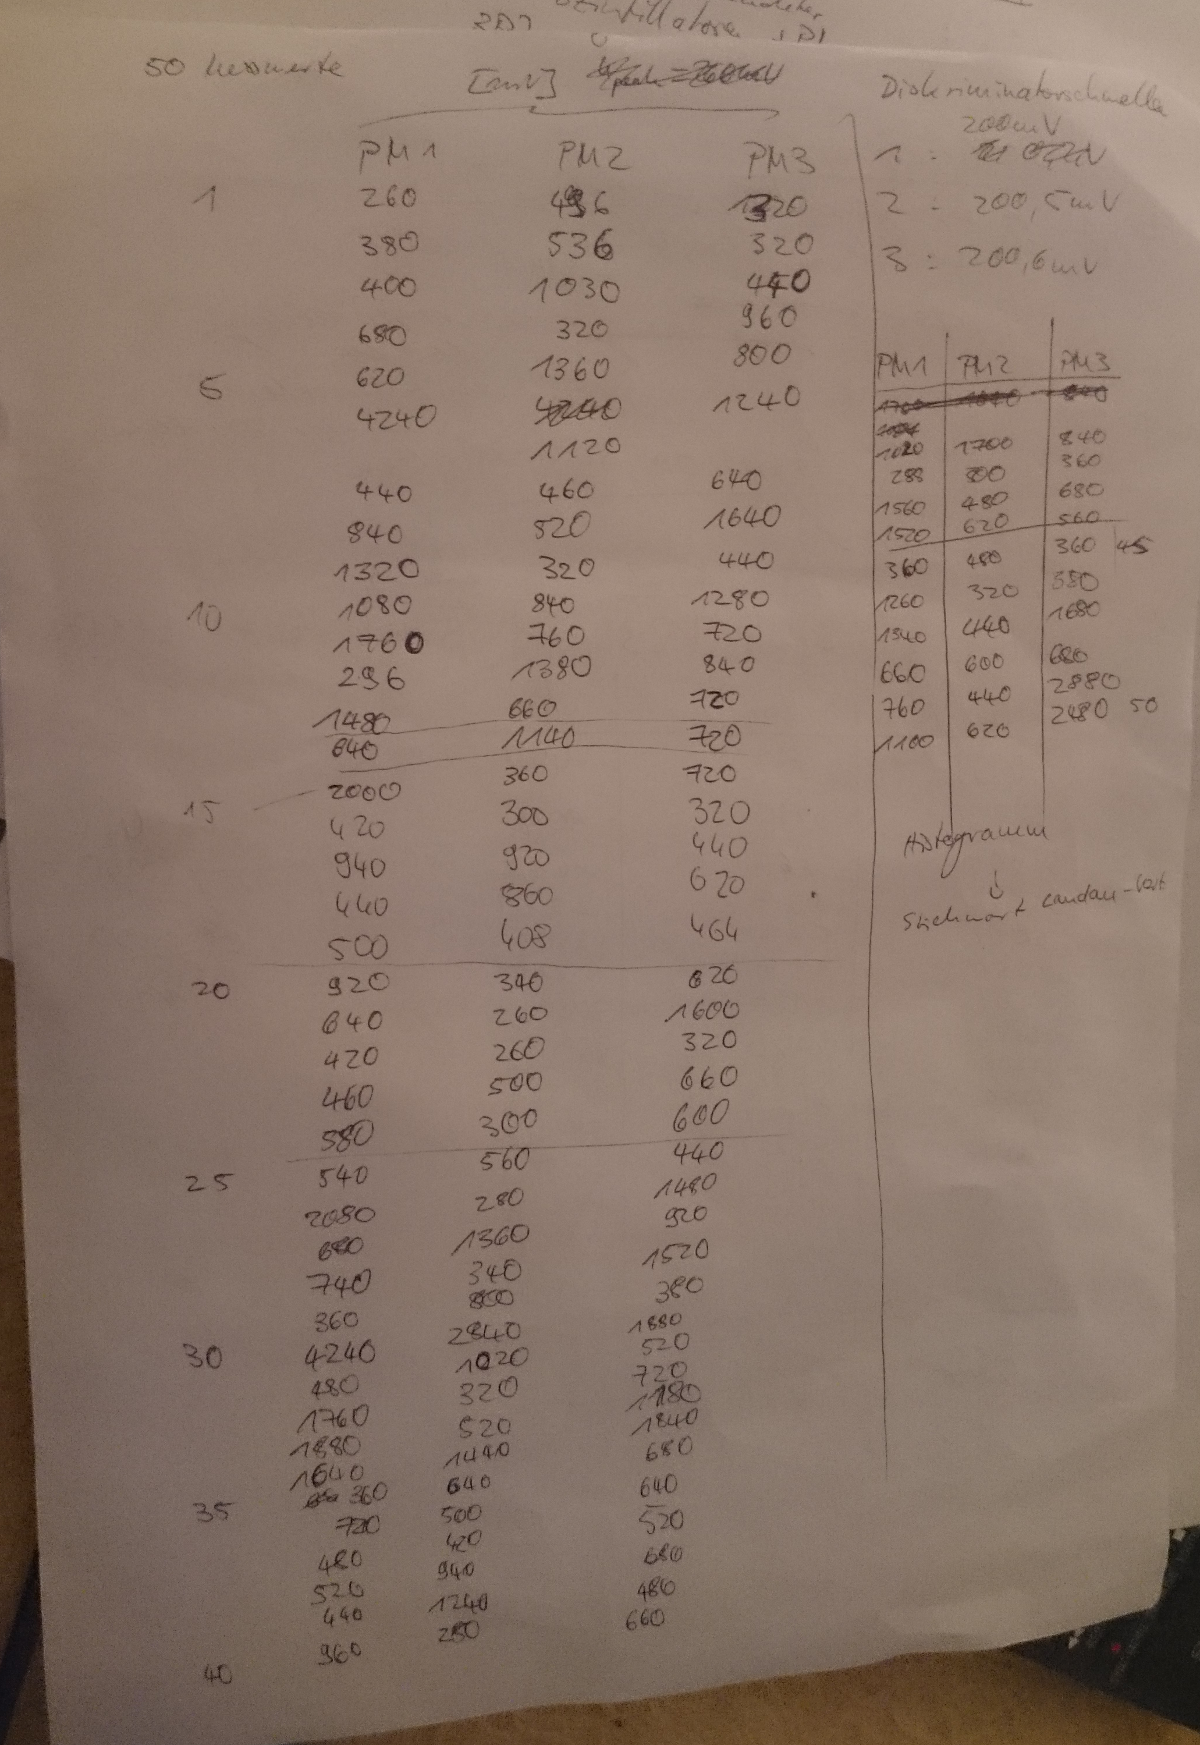
\includegraphics[scale=0.10]{pic/mess2.png}}
    \caption{Messprotokollseiten}
\end{figure}		% Auswertung
\begin{thebibliography}{99}
\bibitem [01] {PA} Technische Universität Dresden,  Institut für Kern- und Teilchenphysik: \textit{Lebensdauer von Myonen - Platzanleitung}. Dresden
\bibitem [02] {pdg} K.A Olive et al. (Particle Data Group), Chin. Phys. C, 38, 090001 (2014) and 2015 update.
\end{thebibliography}



\end{document}
